\chapter*{Demographics of US Elections}
\stepcounter{chapter}

\section{Mapping Data}
\begin{figure}[H]
    \centering
    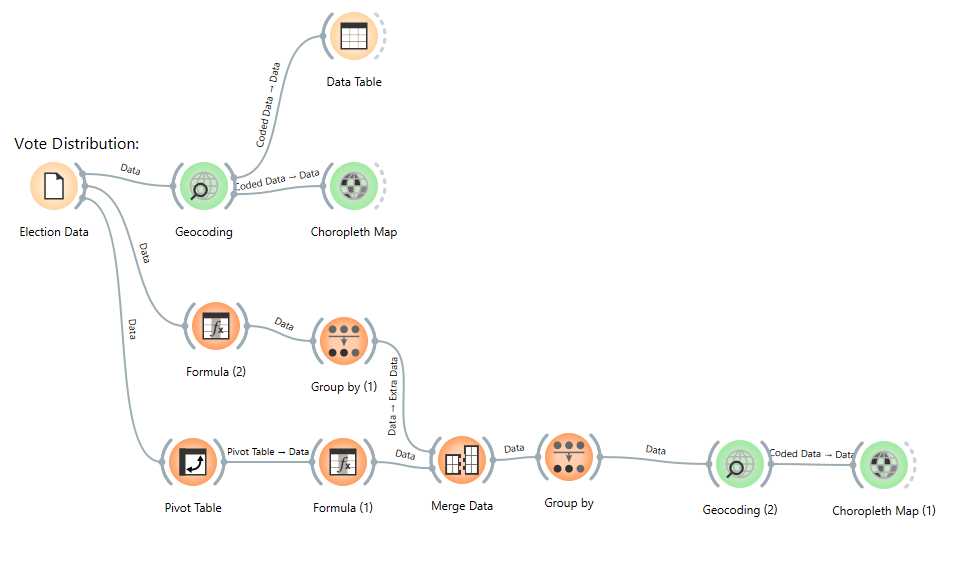
\includegraphics[width=0.7\textwidth]{chapters/part 4 - images/mapping_to_states_nodes.png}
    \caption{Expressing geographical data.}
\end{figure}

\subsection{Election Results:}
\begin{figure}[H]
    \centering
    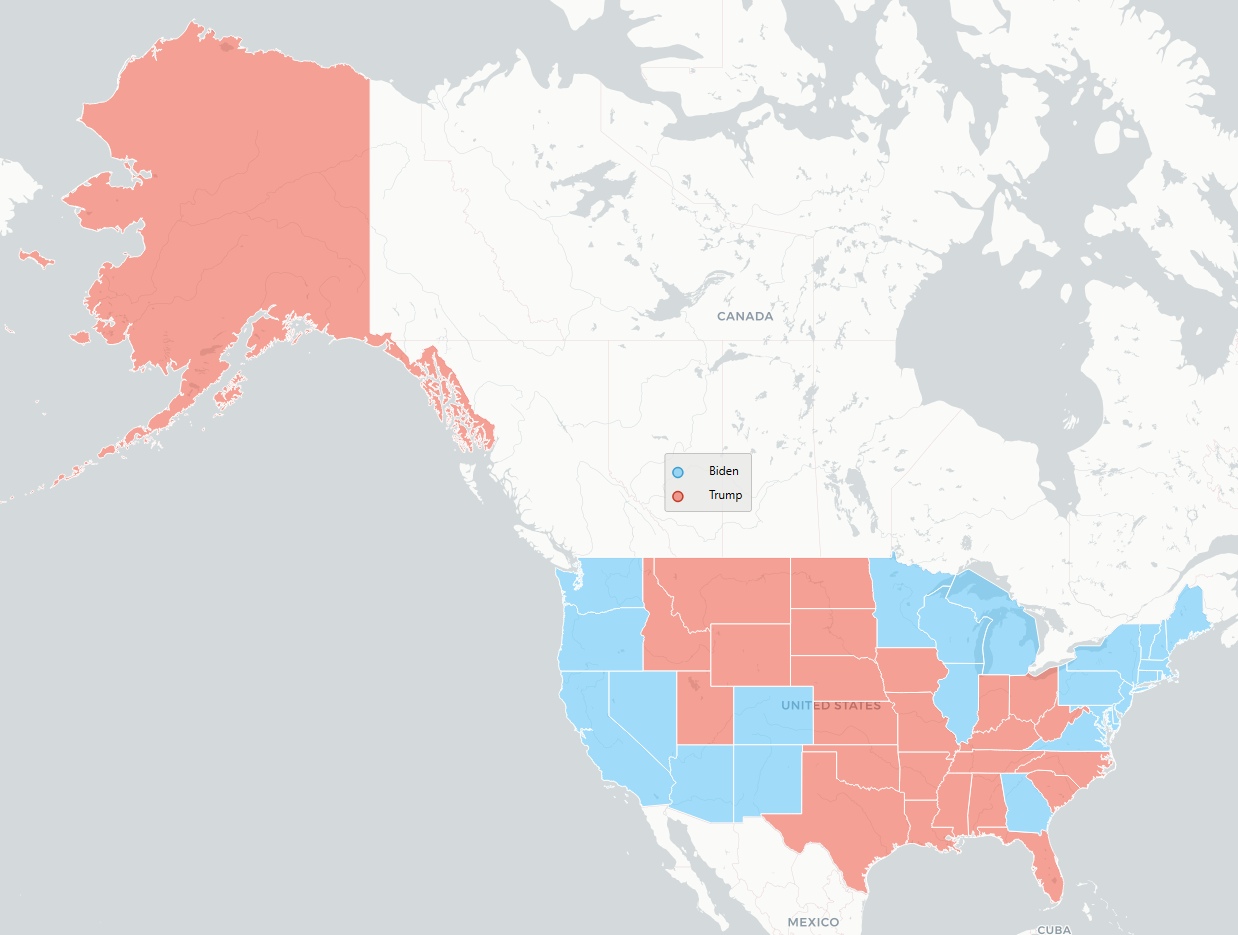
\includegraphics[width=0.7\textwidth]{chapters/part 4 - images/voting (BidenVSTrump).png}
    \caption{Winning Parties between states}
    \label{fig:TvB_votes}
\end{figure}
Figure \ref{fig:TvB_votes} shows which of the top running parties was dominant in which
state in 2020.






\subsubsection{Effect of \textbf{Income} on Voting habits:}
\begin{figure}[H]
     \centering
     \begin{subfigure}[b]{0.45\textwidth}
         \centering
         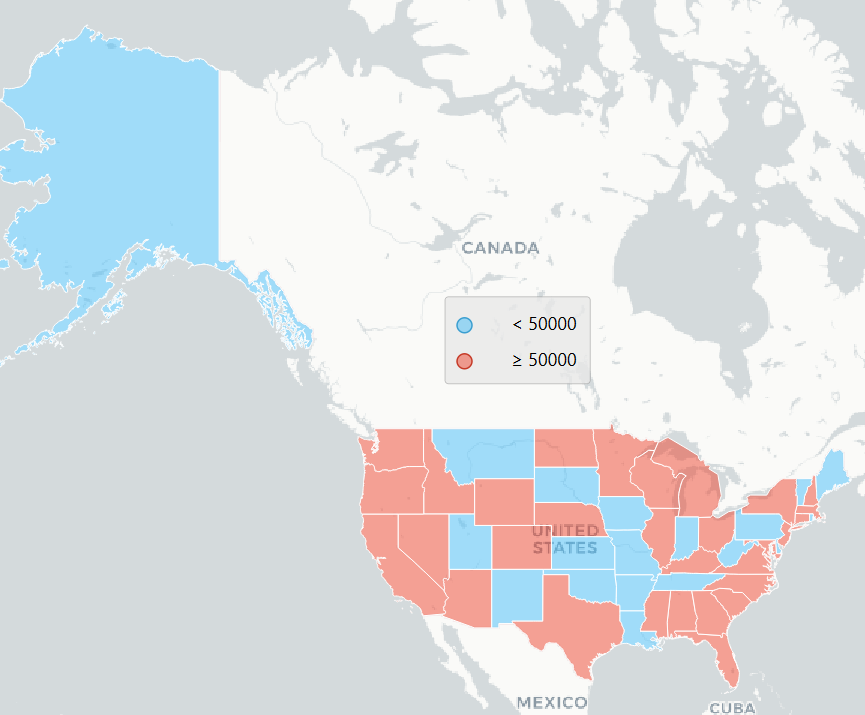
\includegraphics[width=\textwidth]{chapters/part 4 - images/income_level_mean.png}
         \caption{Raw income of voters on average(by state)}
         \label{fig:raw_income_state}
     \end{subfigure}
     \hfill
     \begin{subfigure}[b]{0.45\textwidth}
         \centering
         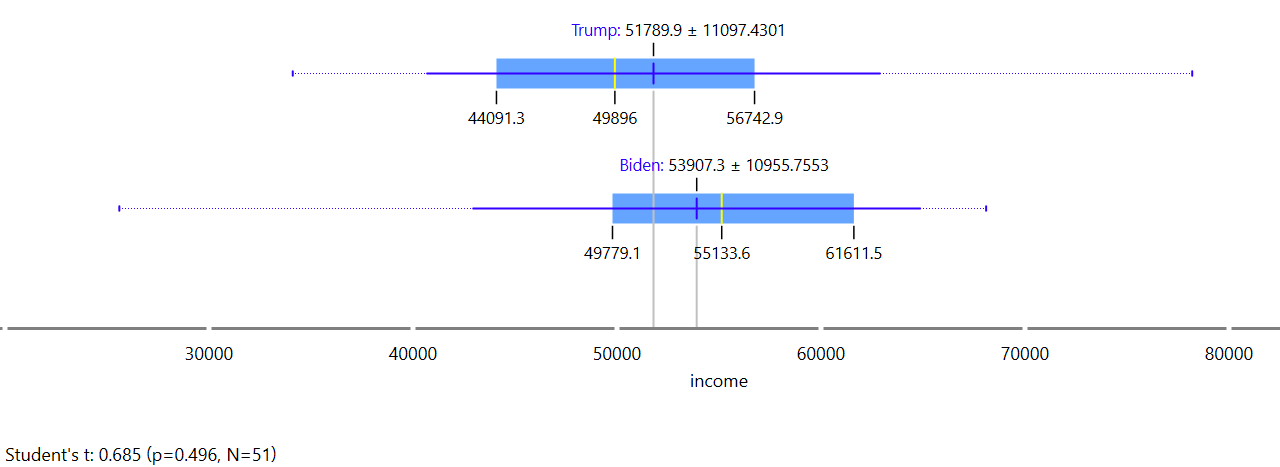
\includegraphics[width=\textwidth]{chapters/part 4 - images/income_spread.png}
         \caption{is the average income high or low?}
         \label{fig:high_low_income_state}
     \end{subfigure}
     \caption{Income distribution between states}
     \label{fig:income_spread_state}
\end{figure}
Initial High vs Low income state decision is not feasible because averaging out state income is diluted by
extreme income which results in $50/51$ states being high-income. This was replaced with a median data split which results in 41/51
states following the pattern of: Biden = High-Income and Trump = Low-Income. With a regression of $\pm0.13$ between raw income and
state vote there is not enough evidence to suggest this is not a result of noise ($p=0.496$).




\subsubsection{\textbf{Education} Correlation in voting:}
\begin{figure}[H]
     \centering
     \begin{subfigure}[b]{0.45\textwidth}
         \centering
         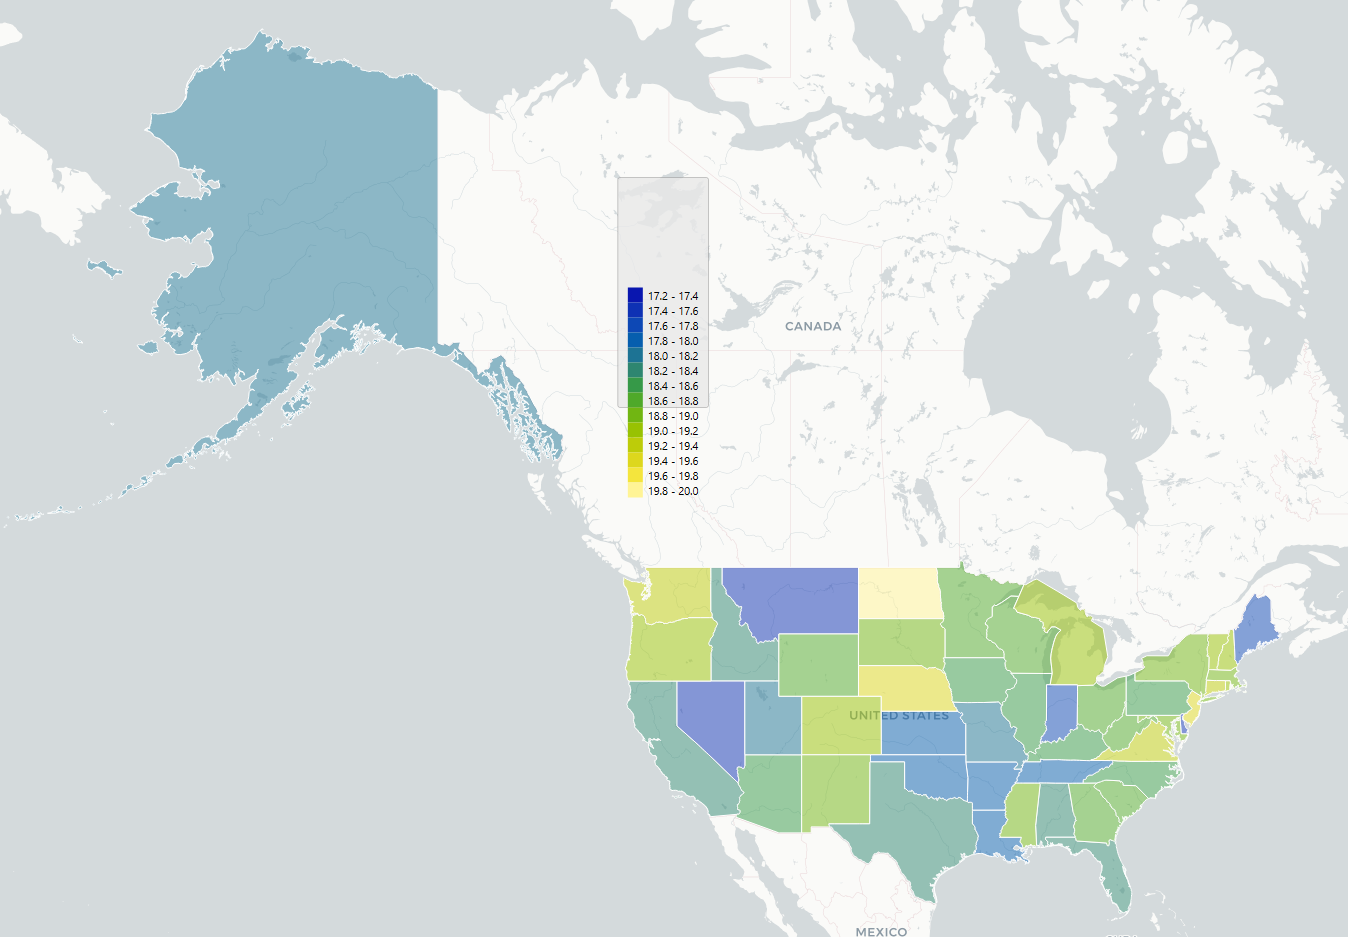
\includegraphics[width=\textwidth]{chapters/part 4 - images/education_mean.png}
         \caption{Education numerical comparisons between states}
         \label{fig:raw_education_states}
     \end{subfigure}
     \hfill
     \begin{subfigure}[b]{0.45\textwidth}
         \centering
         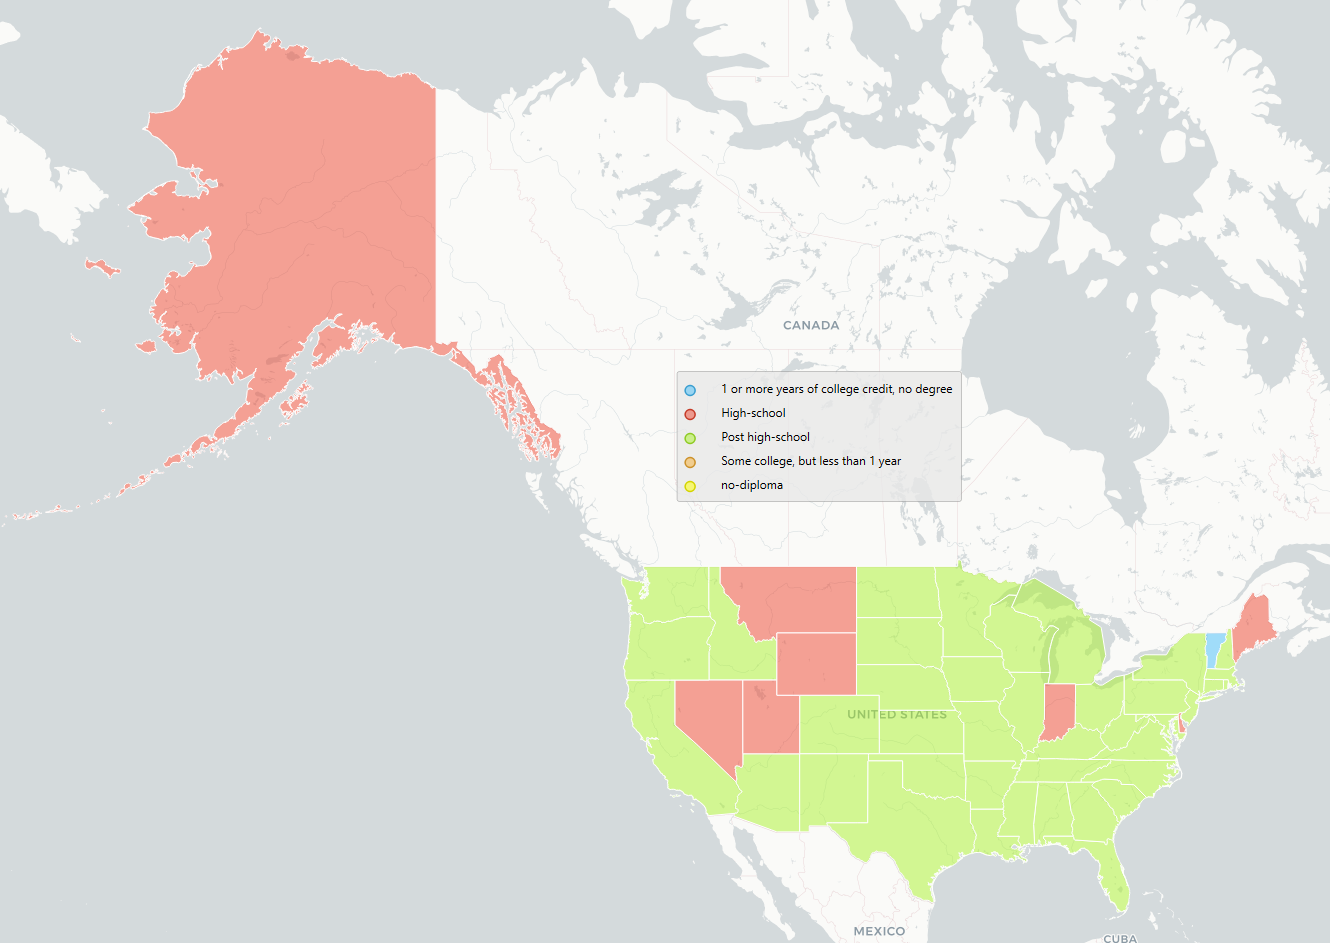
\includegraphics[width=\textwidth]{chapters/part 4 - images/educaiton_level_mean.png}
         \caption{Average eduction level between states}
         \label{fig:edu_level_states}
     \end{subfigure}
     \caption{Education distribution between states}
     \label{fig:edu_states}
\end{figure}
With initial education distribution being unclear as to which candidate they voted for (after
initial comparison), further analysis was required to determine if state-level averages masked
underlying trends in voter attainment.
\begin{figure}[H]
    \centering
    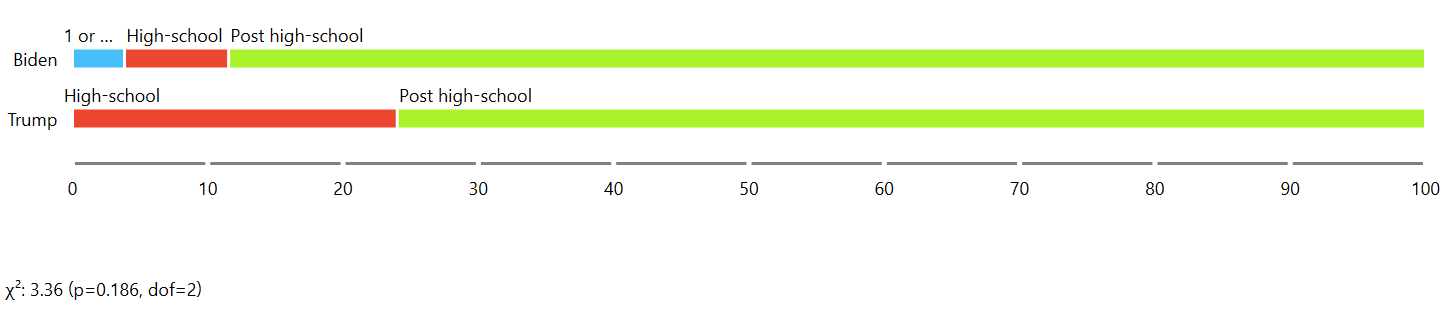
\includegraphics[width=\textwidth]{chapters/part 4 - images/education_spread.png}
    \caption{Distribution of average voters in states for Biden and Trump}
    \label{fig:edu_spread}
\end{figure}
Figure \ref{fig:edu_spread} shows how each candidate's voters were spread by taking a state-wide
average of education level. While a \textbf{visible} reduction in education levels in states that
voted more for Trump there is insufficient evidence that education level correlates to who they
vote for (expressed by $P=0.168$).
\begin{figure}[H]
     \centering
     \begin{subfigure}[b]{0.45\textwidth}
         \centering
         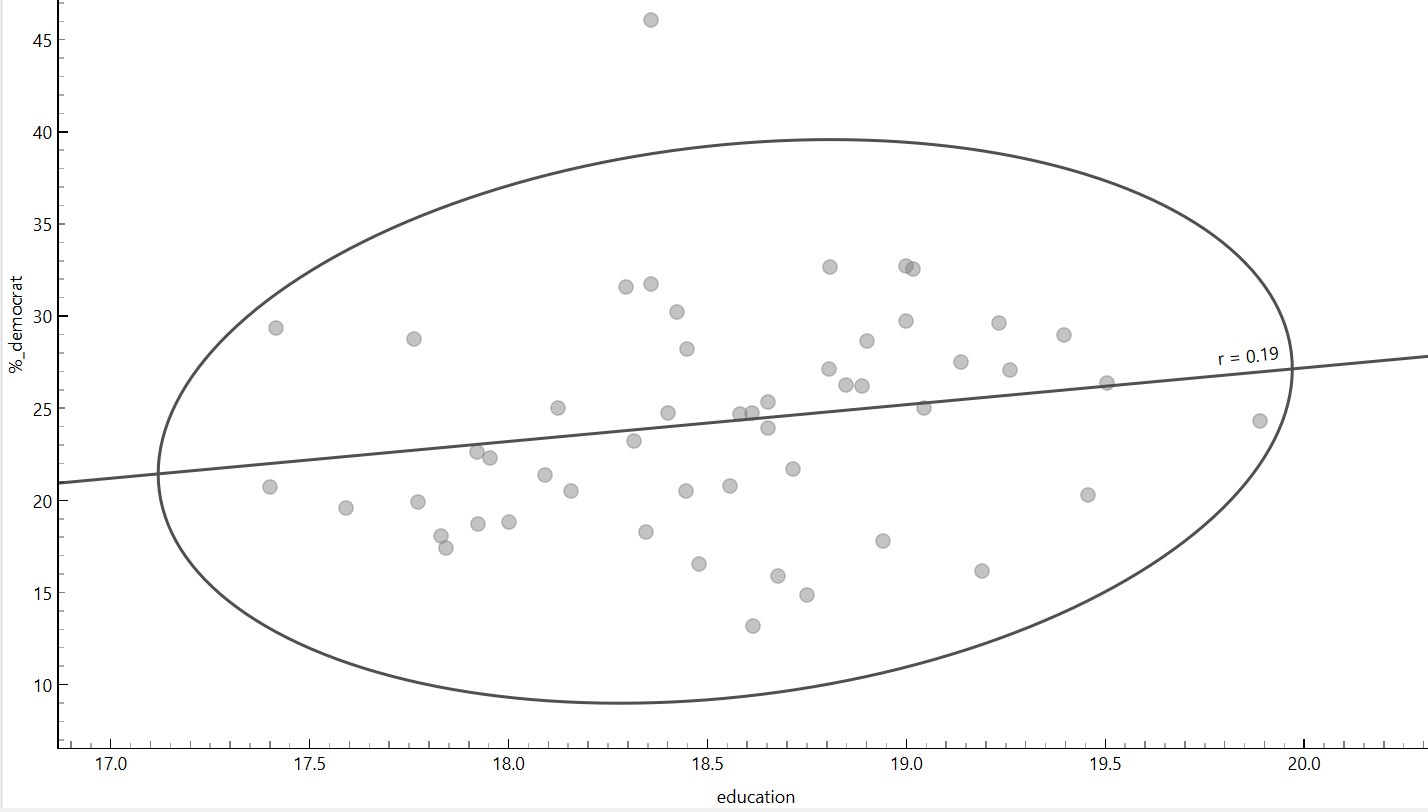
\includegraphics[width=\textwidth]{chapters/part 4 - images/edu_percent_demo.png}
         \caption{Democrat vote \% against education level}
         \label{fig:raw_education_states}
     \end{subfigure}
     \hfill
     \begin{subfigure}[b]{0.45\textwidth}
         \centering
         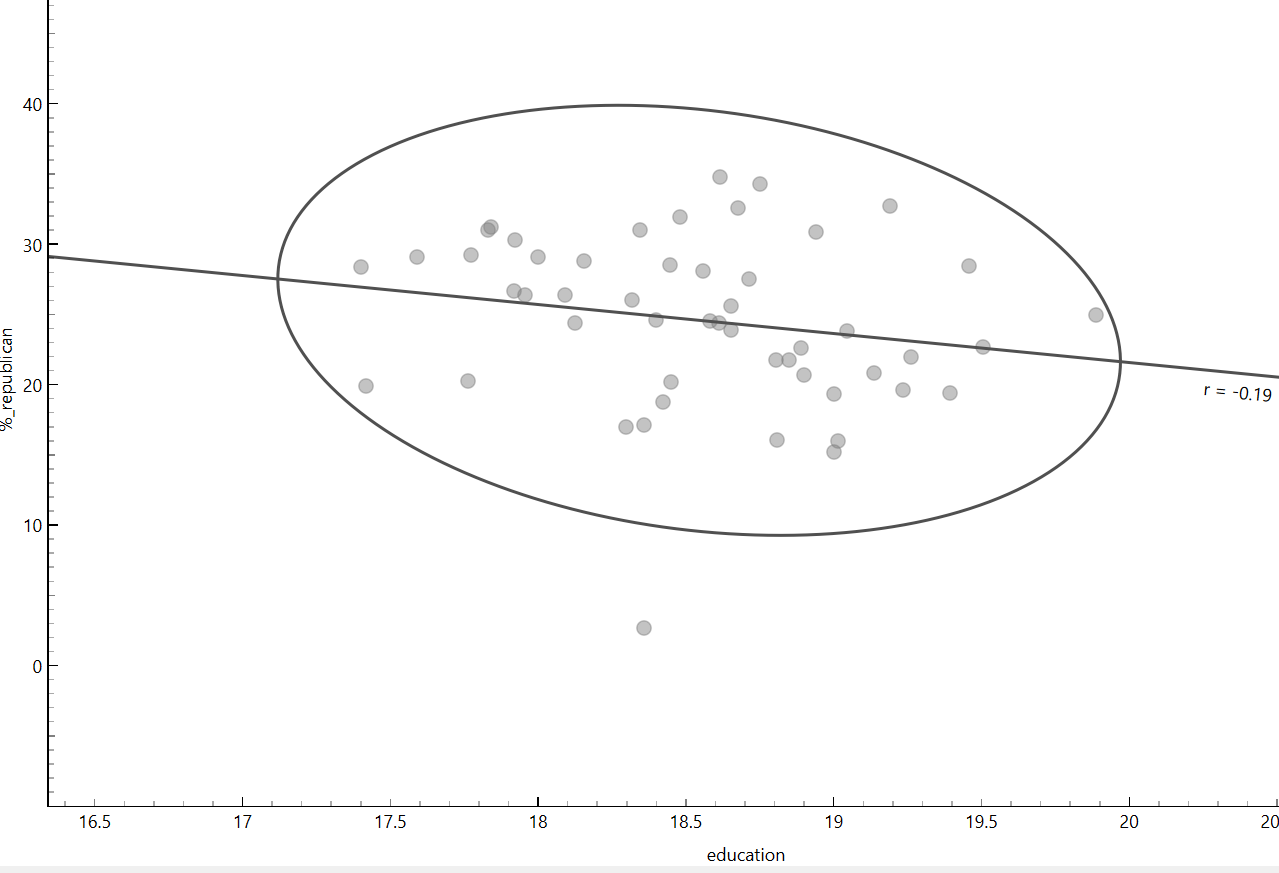
\includegraphics[width=\textwidth]{chapters/part 4 - images/edu_percent_rep.png}
         \caption{Republican vote \% against education level}
         \label{fig:raw_education_states}
     \end{subfigure}
     \caption{Education vs voting bias}
     \label{fig:edu_vote_percent}
\end{figure}
By comparing the percentage distributions however, the effect of varying state size is removed.
As a result, the graphs in figure \ref{fig:edu_vote_percent} shows a weak correlation between the
attributes which suggests it is not the primary driver of voting habits, rather an indication that
those with lower income are more likely to vote Trump (but not exclusively).